\documentclass[12pt]{beamer}
%\usepackage[usenames,dvipsnames]{xcolor}

\usepackage{_defsAndPackages675notation}
\usepackage{_defsAndPackages675beamer}

%\DeclareMathSizes{12}{12}{5}{12}
\newcommand{\parenthetical}[2]{#1  \scriptstyle \alr{( #2)}}
\begin{document}

\title{\alg{Boosting 3: Implementations}}
\subtitle{\classTitle}
%\author{\alg{Darren Homrighausen, PhD}}
%\institute{\classTitle}
\date{}



\begin{frame}
\maketitle

\organization
%
\end{frame}

\begin{frame}[fragile]
\frametitle{Outline}
Now we will discuss two current, popular algorithms and their \alr{R} implementations
\vsp

\begin{itemize}
\item \alr{GBM}
\item \alr{XGBoost}
\end{itemize}
\end{frame}
\transitionSlide{GBM}

\begin{frame}[fragile]
\frametitle{Gradient Boosting Machines (GBM)}
\smallCapGreen{Recall:} AdaBoost effectively uses \alo{forward stagewise} minimization of
the \alo{exponential loss} function

\vsp
\alr{GBM} takes this idea and 
\begin{itemize}
\item generalizes to other loss functions
\item adds subsampling
\item includes methods for choosing $B$
\item reports variable importance measures
\end{itemize}
\end{frame}

\begin{frame}[fragile]
\frametitle{GBM: loss functions}
\begin{itemize}
\item \alr{gaussian}: squared error
\item \alr{laplace}: absolute value 
\item \alr{bernoulli}: logistic 
\item \alr{adaboost}: exponential
\item \alr{multinomial}: more than one class (unordered)
\item \alr{poisson}: Count data
\item \alr{coxph}: For right censored, survival data
\end{itemize}
\end{frame}

\begin{frame}[fragile]
\frametitle{GBM: subsampling}
Early implementations of \alo{AdaBoost} randomly sampled the weights $(w)$

\vsp
This wasn't essential and has been altered to use deterministic weights

\vsp
Friedman (2002) introduced \alg{stochastic} gradient boosting that uses a new subsample
at each boosting iteration to find and project the gradient

\vsp
This has two possible benefits
\begin{itemize}
\item Reduces computations/storage 

\script{But increases read/write time}
\item Can \alo{improve} performance
\end{itemize}
\end{frame}

\begin{frame}[fragile]
\frametitle{GBM: subsampling}
You can expect performance gains when \alo{both} of the following occur:
\vsp

\begin{itemize}
\item There is a small sample size
\item The \alo{base learner} is complex
\end{itemize}
\vsp

This suggests the usual `variance reduction through lowering covariance'' interpretation

\vsp
The effect is complicated, though as subsampling
\begin{itemize}
\item increases the \alo{variance} of each term in the sum
\item decreases the \alo{covariance} of each term in the sum
\end{itemize}
\end{frame}

\begin{frame}[fragile]
\frametitle{GBM: choosing $B$}
There are three built in methods: 
\begin{itemize}
\item \smallCapGreen{Independent test set:} using the \alr{nTrain} parameter to say `use only
this amount of data for training'

\script{Be sure to uniformly permute your data set first.}
\item  \smallCapGreen{Out-of-bag (OOB) estimation:} If \alr{bag.fraction} is $> 0$, then \alr{gbm}
use  OOB at each iteration to find a good $B$

\script{Note: OOB tends to select a too-small $B$}
\item \smallCapGreen{$K$-fold cross validation (CV):}  It will fit \alr{cv.folds}+1 models

\script{The `+1' is the fit on all the data that is reported}
\end{itemize}
\end{frame}

\begin{frame}[fragile]
\frametitle{GBM: variable importance measure}
For tree-based methods, there are two \alg{variable importance measures}:

\begin{itemize}
\item \alr{relative.influence}
\item \alr{permutation.test.gbm}

\script{This is currently labeled experiemental}
\end{itemize}

\vsp

These have similar definition relative to \alb{bagging}, however they use \alo{all} of the data instead of the OOB

\end{frame}

\begin{frame}[fragile]
\frametitle{GBM: sample code}
\begin{blockcode}
gbm(Ytrain~.,data=Xtrain, 
    distribution="bernoulli", 
    n.trees=500,        
    shrinkage=0.01,
    interaction.depth=3,     
    bag.fraction = 0.5,         
    n.minobsinnode = 10,  
    cv.folds = 3,               
    keep.data=TRUE,    
    verbose=TRUE,             
    n.cores=2)                   
    \end{blockcode}
\end{frame}

\begin{frame}[fragile]
\frametitle{GBM: Figures}
\begin{figure}
\centering
\includegraphics[width=2.85in,trim=0 0 0 50,clip]{../figures/gbmMultiCore} \\
\includegraphics[width=1.85in,trim=0 0 0 50,clip]{../figures/gbmCVOOB}
\end{figure}
\end{frame}


\begin{frame}
\frametitle{Distributed computing hierarchy}
\begin{columns}[T]
    \begin{column}{.40\textwidth}

\begin{center}
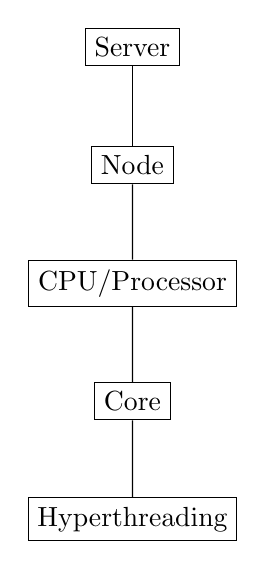
\begin{tikzpicture}
    \tikzstyle{every node}=[rectangle,draw]
    \tikzstyle{level 1}=[sibling distance=39mm] 
    \tikzstyle{level 2}=[sibling distance=23mm]     
    \node {Server}
       child { node {Node}
        child { node {CPU/Processor}
        	child { node {Core}
	  child { node {\alb{Hyperthreading}}}	  
	  }
	}
        }
         ;
\end{tikzpicture}
\end{center}
  \end{column}
    \begin{column}{.60\textwidth}
\smallCapGreen{Example:}  A server might have 

\begin{itemize}
\item 64 nodes
\item 2 processors per node
\item 16 cores per processor
\item \alb{hyper threading}
\end{itemize}


\vsp
The goal is to somehow allocate a \alg{job} so that these resources are
used efficiently

\vsp
Jobs are composed of \alg{threads}, which are specific computations
    \end{column}
  \end{columns}


\end{frame}



\begin{frame}
\frametitle{Hyperthreading}
Developed by Intel, Hypertheading allows for each core to pretend to be two cores
\begin{center}
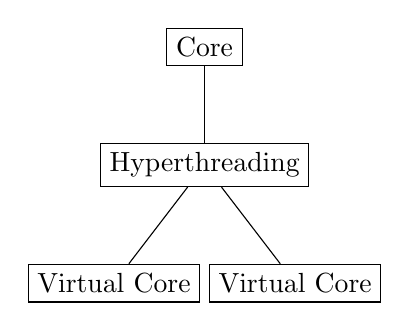
\begin{tikzpicture}
    \tikzstyle{every node}=[rectangle,draw]
    \tikzstyle{level 1}=[sibling distance=39mm] 
    \tikzstyle{level 2}=[sibling distance=23mm]     
    \node {Core}
         child { node {\alb{Hyperthreading}}
           child { node {Virtual Core}}
           child { node {Virtual Core}}
         }
       	  
         ;
\end{tikzpicture}
\end{center}

\vsp
This works by trading off computation and read-time for each core
\end{frame}


\begin{frame}[fragile]
\frametitle{Boosting: Learning slow}
It is best to set the \alo{learning rate} at a small number.

\vsp
This is usually calibrated by the computational demands of the problem.  

\vsp
A good strategy is to pick a number, say .001

\vsp
Run with \alr{n.trees} relatively small and see how long it takes

\vsp
Keep adding trees with \alr{gbm.more}.  If this is taking too long, increase the learning rate
\end{frame}

\transitionSlide{XGBoost}

\begin{frame}[fragile]
\frametitle{XGboost}
This stands for:
\vsp

\smallCapGreen{Extreme Gradient Boosting}

\vsp
It has some advances related to \alr{gbm}
\end{frame}

\begin{frame}[fragile]
\frametitle{XGboost: Advances}
\begin{itemize}
\item \smallCapGreen{Sparse matrices:} Can use sparse matrices as inputs 

\script{In fact, it has its own matrix-like data structure that is recommended}
\item \smallCapGreen{OpenMP:} Incorporates OpenMP on Windows/Linux 

\script{OpenMP is a \alg{message passing} parallelization paradigm for shared memory parallel programming}

\item \smallCapGreen{Loss functions:} You can specifiy your own loss/evaluation functions

\script{You need to use \alr{xgb.train} for this}
\end{itemize}
\end{frame}
\end{document}

\transitionSlide{Additional topics}
\begin{frame}[fragile]
\frametitle{Tree complexity}
The \alg{base} classifier's complexity must be fixed

\vsp
As previously stated, it is usually chosen to be $M \in \{4,\ldots,8\}$

\vsp
This choice controls the number of \alo{interactions} available to the tree, and hence to boosting

\vfill

\end{frame}

\end{document}
